\multiproblem{1}{
By using the Method of Joints, solve for the support forces and the tension/compression in each rod in the following truss structures:
    \begin{enumerate}
        \item Roof Truss: \hfill
        \begin{center}
        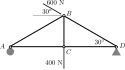
\includegraphics[scale=2]{mj_1.pdf}
        \end{center}
        \item Howe Roof Truss: \hfill
        \begin{center}
        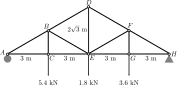
\includegraphics[scale=2]{mj_2.pdf}
        \end{center}
        \item Pratt Roof Truss: \hfill
        \begin{center}
        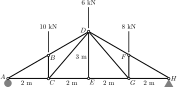
\includegraphics[scale=2]{mj_3.pdf}
        \end{center}
        \item \hfill
        \begin{center}
        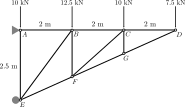
\includegraphics[scale=2]{mj_4.pdf}
        \end{center}
        \item \hfill
        \begin{center}
        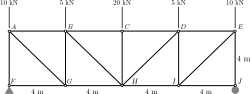
\includegraphics[scale=2]{mj_5.pdf}
        \end{center}
        Hint: use symmetry to save calculation time.
    \end{enumerate}
}

\multiproblem{best}{
Suppose we want to make a roof and need to choose a truss type. We consider three options: the simple roof truss, the Howe Roof truss and the Pratt Roof truss, as shown below. The rods that make the truss can support a given maximum tension/compression, denoted $T_{\text{max}}$. If the tension in any rod exceeds $\pm T_{\text{max}}$ then the rod is expected to fail (break). We want our roof truss to support a load $W$ at the central section (without breaking!). 
\begin{center}
        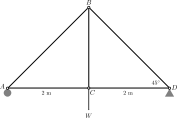
\includegraphics[scale=2]{roof.pdf}
        \end{center}
        \begin{center}
        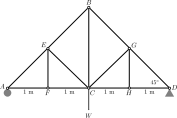
\includegraphics[scale=2]{howe.pdf}
        \end{center}
        \begin{center}
        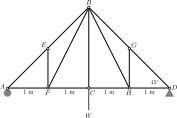
\includegraphics[scale=2]{pratt.pdf}
        \end{center}
\begin{enumerate}
 \item Find the tension in each rod in each truss as a function of the load $W$.
 \item Which truss style supports the largest load $W$ if $T_{\text{max}}$ is the same in each case?
 \item Suppose that we want to minimise the total cost of the roof and hence the truss structure. The cost of a rod is proportional to its length but also to its strength since we can make the rods thicker and stronger by using more material. Assume that the cost of each rod is given by $C=T_{\text{max}}L$ where $T_{\text{max}}$ is the maximum load that the rod can support and $L$ is the length of the rod. Which truss style can support the biggest load for a given price
 \begin{enumerate}
     \item if all rods must be the same strength (have the same $T_{\text{max}}$)?
     \item if we can make some rods stronger than others (having different $T_{\text{max}}$ for each rod)?
 \end{enumerate}
\end{enumerate}

}

\multiproblem{2}{
The Method of Sections allows us to find the forces in specific rods more efficiently. It is generally a good idea to cut the truss through the rods with unknown forces.
    \begin{enumerate}
        \item Using the Method of Sections:
        \begin{enumerate}
        \item Verify the value of $T_{BD}$ and $T_{BE}$ for the truss in 1 (b).
        \item Verify the value of $T_{DG}$ for the truss in 1 (c).
        \item Verify your values for $T_{CF}$ and $T_{BC}$ for the truss in 1 (d). 
        \item Verify your values for $T_{BC}$, $T_{BH}$ and $T_{GH}$ for the truss in 1 (e). 
        \end{enumerate}
        \item Find $T_{BC}$, $T_{CE}$ and $T_{EF}$. \hfill
        \begin{center}
        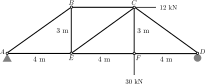
\includegraphics[scale=2]{ms_1.pdf}
        \end{center}
        \item Find $T_{BD}$, $T_{BE}$ and $T_{CE}$. \hfill
        \begin{center}
        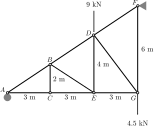
\includegraphics[scale=2]{ms_2.pdf}
        \end{center}
        \item Find $T_{BH}$ and $T_{CG}$. \hfill
        \begin{center}
        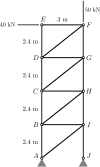
\includegraphics[scale=2]{ms_3.pdf}
        \end{center}               
        \item Find $T_{DF}$, $T_{FG}$ and $T_{GI}$. (Hint: Identify all zero-force rods before you make the cut. The easiest way to find these is to begin by considering the force balance at joint $K$.) \hfill
        \begin{center}
        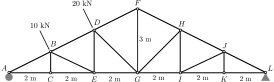
\includegraphics[scale=2]{ms_4.pdf}
        \end{center}        
    \end{enumerate}
}

\multiproblem{3}{
We would like to build a bridge across a ravine. The truss structure of the bridge is as shown below. The truss can be thought of as comprising of $2N$ sub-structures of width $l$ - for instance, in the bridge below $N=3$. The length of the bridge is therefore given by $d=2Nl$.
        \begin{center}
        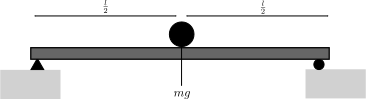
\includegraphics[scale=1.5]{bridge.pdf}
        \end{center} 
       \begin{enumerate}
         \item Using any method you choose find the tension/compression in each rod as a function of $W$ for the bridge shown above. (It might be a bit easier to use Method of Sections.)
         \item Now consider the general case, where the bridge is composed of $N$ sub-structures. By using the Method of Sections, find tension/compression in each rod as a function of $N$ and $W$.
         \item The maximum tension in any rod is denoted $T_{\text{max}}$. By considering the largest load $W$ that can be supported for a given $T_{\text{max}}$ for different $N$, show that the strongest truss structure for the bridge is the simple Roof Truss.
         \item Suppose that the cost of the bridge is directly proportional to the total length of the rods used. Show that for a bridge of length $d$ the total length of the rods is given by
         \begin{equation*}
          2(3+\sqrt{2})-\frac{3}{2N}d.
         \end{equation*}
	 Hence show that the roof truss structure is the cheapest.
	 \item In practice why is this design not always the best?
        \end{enumerate}
}